% 2D Scalar Produces of a Translation
%
% File:         2d-scalar-products-of-translation.tex
% Author:       Bob Walton (walton@acm.org)
% Date:      	Sun Dec 23 05:47:27 EST 2012
  
\documentclass{minimal}
\usepackage[paperheight=3in,paperwidth=2in,
            height=3in,hoffset=0.05in,
	    voffset=0.05in,left=0in,width=2in]{geometry}
\usepackage{color}
\usepackage[usenames]{xcolor}
\usepackage{scalefnt}
\usepackage{tikz}
\usetikzlibrary{arrows}
\newcommand{\SMALL}{\scalefont{0.8}}
\begin{document}
\raggedright
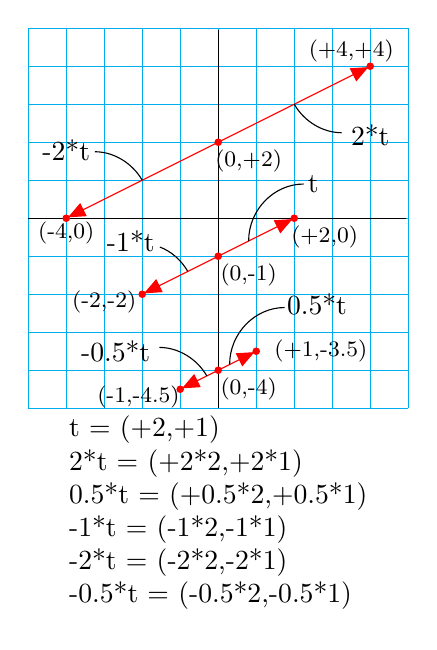
\begin{tikzpicture}[x=0.190in,y=0.190in]
\begin{scope}[yshift=1in,>=triangle 45,shorten >=0.01in]
    \draw[cyan] (-5,-5) grid[step=1] (5,5);
    \draw[black] (-5,0) -- (+5,0);
    \draw[black] (0,-5) -- (0,+5);

    \fill[red] (0,-1) circle(0.1) + (+0.8,-0.5) node[black]{\SMALL(0,-1)};
    \draw[red,->] (0,-1) -- (+2,0);
    \draw[black] (0.8,-0.6) arc(180:90:1.5);
    \draw[black] (2.5,0.9) node{t};
    \fill[red] (+2,0) circle(0.1) + (+0.8,-0.5) node[black]{\SMALL(+2,0)};
    \draw[red,->] (0,-1) -- (-2,-2);
    \draw[black] (-0.8,-1.4) arc(30:70:1.5);
    \draw[black] (-2.3,-0.6) node{-1*t};
    \fill[red] (-2,-2) circle(0.1) + (-1.0,-0.2) node[black]{\SMALL(-2,-2)};

    \fill[red] (0,+2) circle(0.1) + (+0.8,-0.5) node[black]{\SMALL(0,+2)};
    \draw[red,->] (0,+2) -- (+4,+4);
    \draw[black] (2,3) arc(-150:-90:1.5);
    \draw[black] (4.0,2.2) node{2*t};
    \fill[red] (+4,+4) circle(0.1) + (-0.5,0.4) node[black]{\SMALL(+4,+4)};
    \draw[red,->] (0,+2) -- (-4,0);
    \draw[black] (-2,1) arc(30:90:1.5);
    \draw[black] (-4,1.8) node{-2*t};
    \fill[red] (-4,0) circle(0.1) + (0,-0.4) node[black]{\SMALL(-4,0)};

    \fill[red] (0,-4) circle(0.1) + (+0.8,-0.5) node[black]{\SMALL(0,-4)};
    \draw[red,->] (0,-4) -- (+1,-3.5);
    \draw[black] (0.3,-3.85) arc(180:90:1.5);
    \draw[black] (2.6,-2.25) node{0.5*t};
    \fill[red] (+1,-3.5) circle(0.1) + (+1.7,0) node[black]{\SMALL(+1,-3.5)};
    \draw[red,->] (0,-4) -- (-1,-4.5);
    \draw[black] (-0.3,-4.15) arc(30:90:1.5);
    \draw[black] (-2.7,-3.5) node{-0.5*t};
    \fill[red] (-1,-4.5) circle(0.1) + (-1.1,-0.2) node[black]{\SMALL(-1,-4.5)};
\end{scope}

\begin{scope}
\draw (0,-2.5) node {
    \begin{tabular}{l}
    t = (+2,+1) \\
    2*t = (+2*2,+2*1) \\
    0.5*t = (+0.5*2,+0.5*1) \\
    -1*t = (-1*2,-1*1) \\
    -2*t = (-2*2,-2*1) \\
    -0.5*t = (-0.5*2,-0.5*1) \\
    \end{tabular}
    };
\end{scope}
\end{tikzpicture}
\end{document}


